\documentclass[oneside,a4paper,12pt]{article}
\usepackage{graphicx}
\usepackage[section]{placeins}
\usepackage{listings}
\graphicspath{{~/templates/}, {../images/}, {../images/annotated/}}

\makeindex
\begin{document}
	\begin{titlepage}
		\includegraphics[width=4cm]{logopopo.png}
		\hspace*{\fill}
		\includegraphics[width=6cm]{univlille.png}
		
		\begin{center}
			\vspace{1cm}
			\textbf{TP Traitemnent du Signal}\\
			\textbf{Estimation numérique des signaux aléatoires}\\
			\vspace{1cm}
			\textbf{Valentin DOSIAS, Maxence NEUS}\\
			\vspace{3cm}
			%\includegraphics[width=13cm]{titlepage.png}\\
			\vspace{\fill}
			\textbf{Janvier 2022}\\
		\end{center}
	\end{titlepage}
	
	\tableofcontents
	\vspace*{\fill}
	
	\section{Introduction}
	
	Les signaux aléatoires jouent un rôle majeur dans le traitement de signal. Dans la plupart des cas pratiques, ces signaux sont présents sous la forme de bruit dans l’information que nous voulons transmettre. Il n’existe pas de description analytique permettant de traduire l'évolution temporelle des signaux aléatoires. C’est essentiellement des propriétés statistiques qui nous permettent de les caractériser.\\
	Dans la première partie du TP, nous allons comparer avec les lois théoriques, les distributions expérimentales calculées sur des signaux aléatoires stationnaires délivrés par un générateur de bruit.\\
	Dans la seconde partie du TP, nous allons essayer de retrouver, par l’analyse spectrale et par l’analyse fréquentielle, un signal périodique mélangé au bruit. 
	\newpage
	
	\section{Etude statique du bruit}
	
	\subsection{Etude du bruit gaussien}
	
	Pour avoir un bruit gaussien, nous utilisons un générateur de bruit. Nous le réglons pour avoir un bruit gaussien de bande passante 5 kHz. L’atténuateur est réglé à 0 dB, nous centrons ensuite le bruit sur l’écran de l’oscilloscope.\\
	Nous avons relevés les valeurs suivantes :
	\begin{itemize}
		\item[Vmoy] = -120mV
		\item[Veff] = 1.3 V
	\end{itemize}
	Pour relever les caractéristiques statistiques, nous devons choisir différents paramètres. 
	Dans un premier temps, nous prenons une base de temps de 10 ms et faisons une acquisition de 50 points. Nous obtenons l’histogramme ci-dessous.\\
	
	\begin{figure}[h]
		\centering
		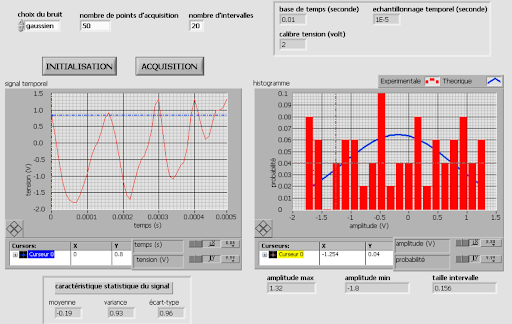
\includegraphics[width=11cm]{fig1.PNG}
		\caption{gaussien 50 points}
	\end{figure}


	Nous obtenons d’abord notre bruit dans le domaine temporel (graphique de gauche). Le graphique de droite est le graphique de bruit dans le domaine probabiliste. La courbe bleue sur le graphique de droite, nous montre la loi de probabilité théorique que nous devrions obtenir et en rouge nous avons nos résultats en pratique. Nous voyons clairement que l’histogramme ne suit pas du tout la loi théorique.\\
	Nous allons modifier les nombres de points d’acquisitions pour voir si cela améliore nos résultats. Nous allons donc faire les mêmes relevés mais cette fois avec 1000 points et 10000 points d’acquisition. Les relevés suivants sont respectivement pour 1000 et 10000 points.
	\begin{figure}[h]
		\centering
		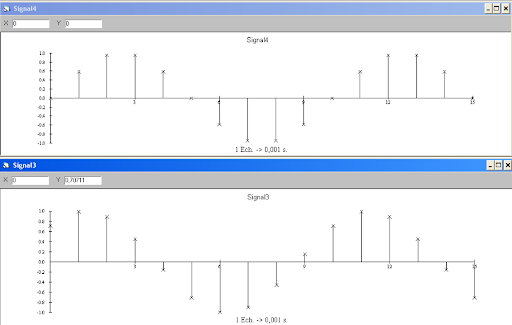
\includegraphics[width=10cm]{fig2.png}
		\caption{gaussien 1000 points}
	\end{figure}
	\begin{figure}[h]
		\centering
		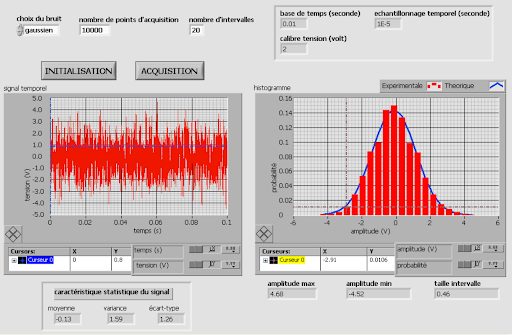
\includegraphics[width=10cm]{fig3.png}
		\caption{gaussien 10000 points}
	\end{figure}

	\newpage
	Nous voyons déjà dans les deux cas que nos relevés temporels ressemblent bien plus à ce que nous pouvons observer sur l’oscilloscope. Dans le domaine fréquentiel, nous observons pour 1000 points une certaine différence pour certaines colonnes de l’histogramme soit en dessous soit au-dessus de la courbe théorique. Pour 10000 points, ces écarts entre les colonnes et la courbe théoriques sont plus faibles. Ainsi nous pouvons conclure que plus le nombre de points d’acquisitions augmentent plus la représentation expérimentale s’accorde avec la représentation théorique. En effet , plus le nombre de points augmentent , plus l'histogramme tend à ressembler à la courbe de la loi de distribution de Gauss. Avec 50 points, certaines mesures sont perdues, donc le signal est dénaturé tandis qu’avec 10000 points, le bruit est mieux mesuré donc mieux représenté dans le logiciel de mesure.\\
	
	Nous allons maintenant faire varier la base de temps pour se rendre compte de son influence sur les résultats que nous obtenons. Nous changeons la base de temps à 0.2ms. Nous obtenons les relevés suivants pour 1000 et 10000 points.\\
	
	\begin{figure}[h]
		\centering
		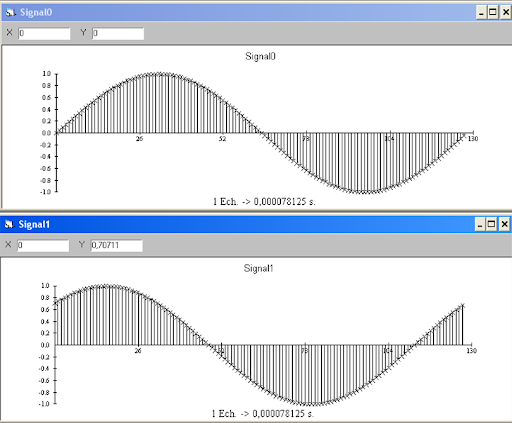
\includegraphics[width=12cm]{fig4.png}
		\caption{0.2 ms 1000 points}
	\end{figure}
\newpage

	\begin{figure}[h]
		\centering
		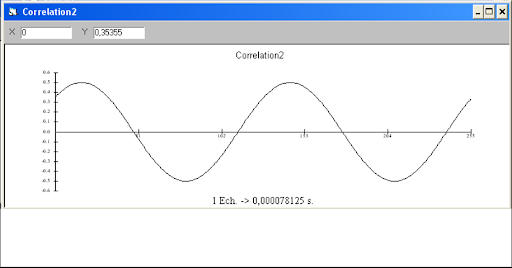
\includegraphics[width=12cm]{fig5.png}
		\caption{0.2 ms 10000 points}
	\end{figure}
	
	Il est possible de faire varier la base de temps avec l’oscilloscope. Pour la figure à 1000 points les résultats ne sont pas du tout en accord avec la théorie. Nous voyons qu’à nombre de points égale, les résultats pratiques sont moins en accord avec les résultats théoriques que pour une base de 10 ms. Ainsi, plus la base de temps est élevée, plus nous avons une variété d’amplitude dans nos mesures alors qu’avec une plus petite base de temps, nos valeurs sur les amplitudes vont être plus précises mais moins nombreuses. Il faut donc faire un compromis en fonction de notre signal sur le nombre de points à capturer et sur la taille de fenêtre temporelle.\\
	La taille de la fenêtre va être à choisir en fonction de la bande passante du signal pour voir si ce que l’on observe est représentatif du bruit et le nombre de points va surtout influer sur la précision voulue sur nos résultats. Un trop grand nombre de points peut amener à un temps de calcul trop important.
	
	\newpage
	\subsection{Etude du bruit uniforme}
	
	Nous allons maintenant générer un bruit uniforme dont l’horloge est réglée à 20µs. Nous avons choisi une base de temps de 0.02 seconde pour observer la totalité du signal et avons choisi un nombre de points très important pour avoir la meilleur précision possible sur notre résultat. Nous avons choisi 10000 points d’acquisition, avec 1000 points d’acquisition les écarts étaient trop importants entre la courbe théorique bleu et les colonnes de l'histogramme. Comme nous l’avons vu dans les parties suivantes, pour obtenir un meilleur résultat il aurait fallu faire la moyenne sur plusieurs acquisitions.
	
	\begin{figure}[h]
		\centering
		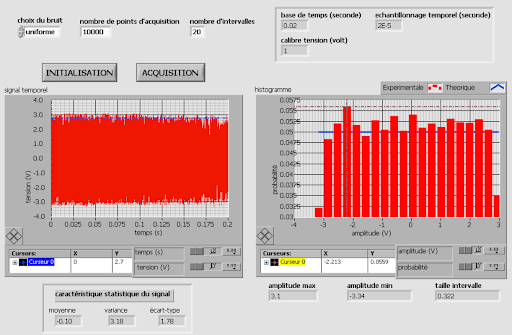
\includegraphics[width=12cm]{fig6.png}
		\caption{bruit uniforme 10000 points}
	\end{figure}

	\newpage
	\section{Etude des estimateurs spectraux}
	\subsection{Préparation}
	
	A partir de la transformée de Fourier d’un signal nous pouvons calculer sa densité spectrale de puissance en faisant le carré du module de sa transformée de Fourier divisée par le temps d’intégration soit $ T_{0} $. Nous avons donc :
	$$ DSP = \frac{|T|^{2}}{T_{0}} $$
	
	Pour calculer la puissance à partir de la DSP, il faut faire intégrer de moins l’infini à plus l’infini la densité spectrale de puissance. Soit S(f) la densité spectrale de puissance d’un signal
	$$ P = \int_{-\infty}^{+\infty} S(f)df $$
	
	\subsection{Periodigramme simple}
	
	Le périodogramme nous permet de calculer la densité spectrale des échantillons d’un signal à partir de la transformée de Fourier de celui-ci. Nous allons d’abord générer un bruit de bande passante 5 kHz et d’atténuation 0 dB. Nous allons d’abord faire une acquisition avec seulement le bruit sur 5000 puis 10000 points. 
	\begin{figure}[h]
		\centering
		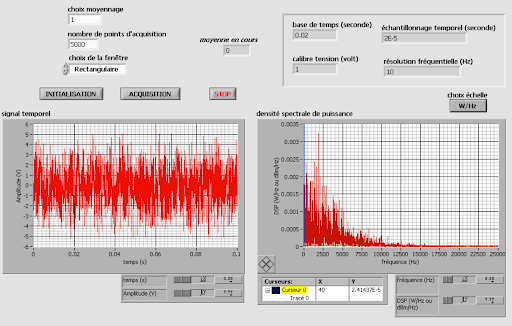
\includegraphics[width=10cm]{fig7.png}
		\caption{5000 points}
	\end{figure}

	\newpage
	\begin{figure}[h]
		\centering
		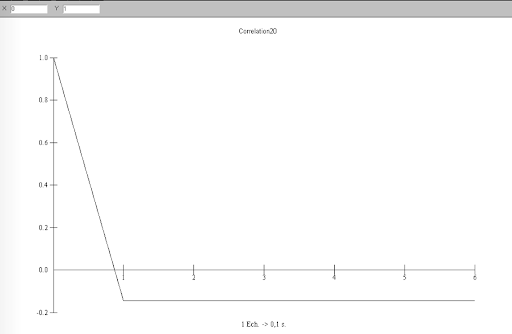
\includegraphics[width=9cm]{fig8.png}
		\caption{10000 points}
	\end{figure}

	Pour un bruit blanc la DSP attendue est une constant sur tout l’axe des fréquences, or il est impossible dans la réalité d’obtenir un bruit blanc, notre bruit généré s’apparente donc à un bruit blanc à bande limitée. L’autocorrélation de ce bruit est donc une porte puisque nous l’observons entre deux fréquences. Ainsi la DSP attendu est donc un sinus cardinal d’ouverture 10 kHz. Nous observons bien  le premier lobe d’un sinus cardinal qui s’annule en 10 kHz.
	\newpage
	Maintenant que nous avons observé notre bruit nous allons le mélanger à un signal sinusoïdal de fréquence 2kHz et d’amplitude 1 Vcc. Nous avons fait l’acquisition sur 5000 points.\\
	\begin{figure}[h]
		\centering
		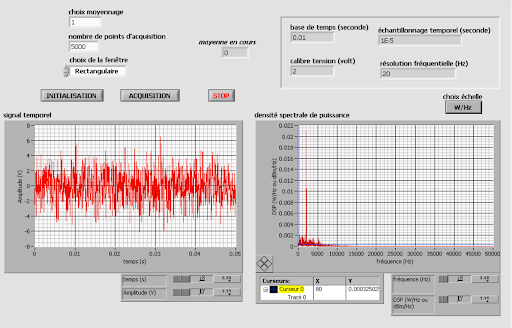
\includegraphics[width=9cm]{fig9.png}
		\caption{Périodogramme du mélange entre le signal harmonique et du bruit gaussien 5000 points sans moyennage}
	\end{figure}

	Nous observons le toujours le premier lobe du sinus cardinal provenant du bruit, nous observons aussi un pic de Dirac à 2 kHz qui correspond bien à la transformée de Fourier de notre signal de fréquence 2 kHz. Plus nous capturons avec un nombre de points élevé, plus ce lobe est compliqué à observer. 

\end{document}